\documentclass[12pt, a4paper]{article}

\usepackage{array}
\usepackage[portuguese]{babel}
\usepackage{chngpage}
\usepackage{float}
\usepackage[a4paper, margin=2cm]{geometry}
\usepackage{graphicx}
\usepackage{hyperref}
\usepackage{setspace}
\usepackage{xcolor}

\title{\Huge \textbf{Computação Gráfica \\ \Large Trabalho Prático -- Fase I}}
\date{2 de março 2025}
\author{Grupo \textbf{\color{red} TODO}}

\begin{document}

\begin{center}
    
\includegraphics[width=0.25\textwidth]{res/cover/EE-C.eps}
\end{center}

\chardef\_=`_
\onehalfspacing
\setlength{\parskip}{\baselineskip}
\setlength{\parindent}{0pt}
\def\arraystretch{1.5}

{\let\newpage\relax\maketitle}
\maketitle
\thispagestyle{empty}

\vspace*{\fill}

\begin{adjustwidth}{-2cm}{-2cm} % These values only need to be large enough to center the table
    \begin{center}
        \begin{tabular}{>{\centering}p{0.25\textwidth}
                        >{\centering}p{0.25\textwidth}
                        >{\centering}p{0.25\textwidth}
                        >{\centering\arraybackslash}p{0.25\textwidth}}
            
\includegraphics[width=3.5cm]{res/cover/A104437.png} &
            
\includegraphics[width=3.5cm]{res/cover/A104348.png} &
            
\includegraphics[width=3.5cm]{res/cover/A90817.png} &
            
\includegraphics[width=3.5cm]{res/cover/A104179.png} \\

            Ana Oliveira & Humberto Gomes & Mariana Cristino & Sara Lopes \\
            A104437      & A104348        & A90817           & A104179
        \end{tabular}
    \end{center}
\end{adjustwidth}

\pagebreak

\begin{abstract}
    \textbf{\color{red} TODO - resumo}
\end{abstract}

\section{\emph{Generator}}

\subsection{Funcionamento do programa}

O programa \texttt{generator} é responsável por gerar modelos 3D de sólidos geométricos, ou seja,
ficheiros com os vértices e as faces triangulares destes sólidos. Nesta fase, o \texttt{generator}
deve ser capaz de gerar as seguintes figuras: planos, cubos, esferas e cones. Além de implementarmos
a geração destas figuras, como funcionalidade adicional, também desenvolvemos um gerador de
cilindros e de tori. As várias possibilidades de uso do comando \texttt{generator} são enumeradas
abaixo:

\begin{verbatim}
./generator plane    <length>      <divisions>                     <file>
./generator box      <length>      <grid>                          <file>
./generator sphere   <radius>      <slices>      <stacks>          <file>
./generator cone     <radius>      <height>      <slices> <stacks> <file>
./generator cylinder <radius>      <height>      <slices> <stacks> <file>
./generator torus    <majorRadius> <minorRadius> <slices> <stacks> <file>
\end{verbatim}

Internamente, o \texttt{generator} começa por interpretar os argumentos dados, saindo com a mensagem
acima em caso de erro. Caso contrário, gera, em memória, os conjuntos de vértices e de faces que
constituem o modelo 3D que, por fim, são escritos para um ficheiro no formato descrito abaixo.

\subsection{Formato \texttt{.3d}}

Decidimos que o formato de saída do \texttt{generator} seria o Wavefront OBJ \cite{wavefront-obj}.
O uso de um formato já existente apresentou diversas vantagens:

\begin{itemize}
    \item Foi possível desenvolver a \texttt{engine} e o \texttt{generator} em paralelo: os
        desenvolvedores do \texttt{generator} não precisavam de ter a \texttt{engine} funcional para
        testar o seu código, visto que já existem diversas ferramentas para visualizar os ficheiros
        OBJ exportados pelo \texttt{generator}.

    \item Foi possível, sem qualquer código adicional, apresentar na \texttt{engine} modelos 3D
        oriundos de ferramentas de modelação, muito mais complexos do que os gerados pelo
        \texttt{generator}.

    \item A forma de representação de faces triangulares neste formato é facilmente mapeável para
        \emph{index buffers} do OpenGL. Deste modo, não seriam necessárias alterações ao
        \texttt{generator} quando estes fossem implementados (algo que já foi feito nesta fase do
        trabalho).
\end{itemize}

O \emph{parser} desenvolvido para este formato suporta apenas o essencial para o funcionamento desta
primeira fase: posições de vértices e constituições de faces triangulares. O formato OBJ é textual,
e representar um vértice é tão simples como ter uma linha começada por um \texttt{v}, ao qual se
seguem as coordenadas do vértice separadas por espaços. O exemplo abaixo representa as coordenadas
$(0, 0.5, 1)$:

\begin{verbatim}
v 0 0.5 1
\end{verbatim}

Faces triangulares são representadas em linhas começadas por um \texttt{f}, ao qual se seguem os
índices dos três vértices da face. É de notar que a contagem dos índices começa em 1, e não em 0.
Por exemplo, para representar uma face triangular, formada pelo primeiro, segundo e terceiro
vértices do ficheiro, tem-se:

\begin{verbatim}
f 1 2 3
\end{verbatim}

\subsection{Cone}
Para gerar um cone temos de indicar o raio da base do cone (radius), a altura do
cone (height), o número de slices, o número de stacks e o caminho relativo para o
ficheiro que iremos criar com os vértices e faces triângulares do cone (file).

Para calcular os vértices e as faces triângulares de um cone, primeiro tivemos
de tomar uma decisão. No enunciado apenas diz que a base do cone deve estar no
plano XZ. Assim, sabemos que a ordenada (y) do centro da base do cone é nula
mas nada nos é dito sobre a abscissa (x) e sobre a cota (z) do centro da base
do cone. Para o cone estar consistente com as restantes figuras e para facilitar
os cálculos, decidimos que a base do cone estaria centrada na origem, ou seja,
teria abcissa e cota nulas.

\subsubsection{Vértices}

Depois, começamos por calcular os vértices do cone.

O primeiro vértice é a origem e o último vértice está localizado no topo do cone,
tendo abscissa e cota nulas e tendo ordenada igual à altura do cone.
$$
P_0 = (0, 0, 0)
\hspace{1cm}
P_n = (0, height, 0)
$$

\begin{figure}[H]
    \centering
    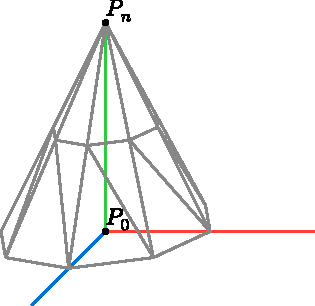
\includegraphics[width=0.4\textwidth]{res/figures/Cone1.pdf}
    \caption{
        Cone gerado, o seu primeiro vértice ($P_0$) e o seu último vértice ($P_n$).
    }
\end{figure}

Também calculamos os restantes vértices. Para cada stack, calculamos X
vértices, sendo X o número de slices.

\begin{figure}[H]
    \centering
    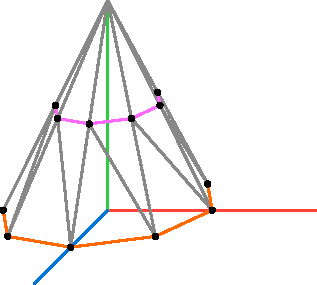
\includegraphics[width=0.4\textwidth]{res/figures/Cone2.pdf}
    \caption{
        Cone com 2 stacks e os vértices (visíveis) calculados em cada stack.
    }
\end{figure}

Como podemos ver pela imagem os vértices calculados para uma stack,
teem todos a mesma ordenada. Podemos obter a ordenada da seguinte forma:
$$
y = \frac{height}{stacks} \times iStack
$$
iStack representa o índice da stack, começando de 0.

Para cada stack, ainda obtemos o raio da circunferência formada pelos vértices dessa stack,
que será usado posteriormente para calcular abcissas e cotas.
Para obter o raio, utilizamos a regra da semelhança de triângulos que nos diz que triângulos
semelhantes teem o comprimento dos lados proporcionais:
$$
newRadius = \frac{(height - y)}{height}\times radius
$$
Depois, ainda numa stack, por cada slice vamos calcular então um vértice.

Já calculamos a ordenada do vértice, agora iremos calcular a abcissa e a cota do
vértice. Para calcular isso, primeiro precisamos de determinar um ângulo.

A circunferência completa tem um ângulo total de $2\pi$ radianos (360°).
Se dividirmos essa circunferência em slices, cada slice terá um ângulo de:
$$
\frac{2 \times \pi}{slices}
$$
Agora, para um slice específico, o ângulo acumulado desde o ponto inicial é:
$$
angle = \frac{(2 \times \pi)}{slices}\times iSlice
$$
iSlice representa O índice do slice, começando de 0.

Isso significa que conforme avançamos pelos slices, o ângulo vai aumentando progressivamente.

Depois com este angulo e com o raio anteriormente obtido, conseguimos calcular a abcissa e
a cota do vértice, usando trignometria:
$$
x = newRadius \times \cos(angle)
$$
$$
z = newRadius \times \sin(angle)
$$
Assim, conseguimos calcular os vértices do cone, sem repetições.

\subsubsection{Faces triângulares}

Depois de termos os vértices, falta calcular as faces triângulares. Primeiro vamos calcular
as faces da base do cone, depois vamos calcular as faces laterais do cone exceto as da
última stack e por fim iremos calcular as faces laterais da última stack.

Em primeiro lugar, calculamos as faces triângulares da base do cone, garantindo que estão viradas
para baixo. Para cada slice, calculamos uma face, que terá sempre como vértices a origem,
outro vértice da base e o vértice que vem a seguir deste.

\begin{figure}[H]
    \centering
    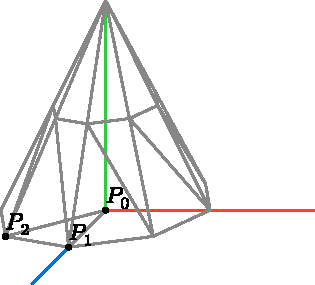
\includegraphics[width=0.4\textwidth]{res/figures/Cone3.pdf}
    \caption{
        Primeira iteração para formar a primeira face da base de um cone com 8 slices e 2 stacks.
    }
\end{figure}

Em segundo lugar, calculamos as faces triângulares laterais do cone, exceto as da última stack
(a stack de maior ordenada), garantindo que estão viradas para fora. Para cada stack, calculamos
$2 \times X$ faces, sendo X o número de slices. Ou seja, numa stack, por cada slice, calculamos
2 faces. A primeira face terá um vértice inicial, o vértice em cima deste e o vértice ao lado do
anterior. A segunda face terá o vértice inicial, o vértice em cima e ao lado desse (na diagonal) e o
vértice ao lado do inicial. Por exemplo, na figura abaixo, a primeira face tem os vértices P1,
P9 e P10 e a segunda face tem os vértices P1, P10 e P2.

\begin{figure}[H]
    \centering
    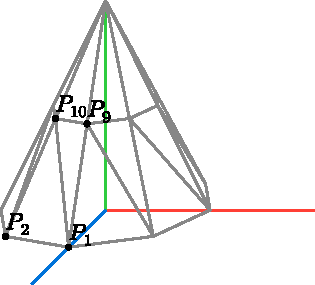
\includegraphics[width=0.4\textwidth]{res/figures/Cone4.pdf}
    \caption{
        Primeira iteração para formar as duas primeiras faces laterais (que
        não são da última stack) de um cone com 8 slices e 2 stacks.
    }
\end{figure}

Em terceiro lugar, calculamos as faces triângulares laterais do cone da última stack, garantindo
que estão viradas para fora. Desta vez, a stack terá apenas X faces, sendo X o número de slices.
Nesta stack, por cada slice, calculamos 1 face. Essa face terá um vértice inicial, o ultimo
vértice de todos (a ponta do cone) e o vértice ao lado do inicial.

\begin{figure}[H]
    \centering
    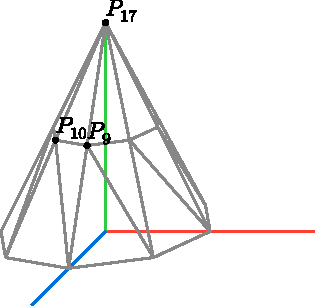
\includegraphics[width=0.4\textwidth]{res/figures/Cone5.pdf}
    \caption{
        Primeira iteração para formar a primeira face da última stack de um cone com 8 slices
        e 2 stacks.
    }
\end{figure}

Temos estas 3 etapas para garantir que não repetimos faces (podiamos ter apenas 2 mas iríamos
repetir faces).

\section{\emph{Engine}}

\textbf{\color{red} TODO - \emph{engine}}

\section{Resultados obtidos}

\textbf{\color{red} TODO - resultados}

\section{Conclusão e Trabalho Futuro}

\textbf{\color{red} TODO - conclusão}

\begingroup
\section{Bibliografia}
\renewcommand{\section}[2]{}

\begin{thebibliography}{9}
    \bibitem{wavefront-obj}
        "Wavefront OBJ File Format Summary."{} FileFormat.Info. Accessed: Mar. 2, 2025. [Online.]
        Available: \url{https://www.fileformat.info/format/wavefrontobj/egff.htm}
\end{thebibliography}
\endgroup

\end{document}
